\documentclass[a4paper, 12pt, notitlepage]{article}
\usepackage[brazil]{babel}
\usepackage[utf8]{inputenc}
\usepackage[hmargin=2cm,vmargin=3cm,bmargin=3cm]{geometry}
\usepackage{enumerate}
\usepackage{graphicx}
\usepackage{mathtools}
\usepackage{physics}
\usepackage{amsmath,amssymb,amsthm}  %pacotes para matemática, opções de indentação, e links
\usepackage{caption}  % caption to minipages
\usepackage{indentfirst}
\usepackage{makeidx}
\usepackage{hyperref}
\hypersetup{colorlinks=false}
\usepackage[T1]{fontenc}
\usepackage{microtype}

\usepackage[sc,osf]{mathpazo}   % With old-style figures and real smallcaps.
\linespread{1.030}              % Palatino leads a little more leading

% Euler for math and numbers
\usepackage[euler-digits,small]{eulervm}
\AtBeginDocument{\renewcommand{\hbar}{\hslash}}

% Latex plots and drawings
\usepackage{tikz}
\usetikzlibrary{arrows.meta, angles, quotes}
\tikzset{>={Latex[width=3mm,length=3mm]}}  %setas mais visíveis no tikz
\usepackage{pgfplots}
\usepgfplotslibrary{fillbetween}

% some useful math shortcuts
\newtheorem{lema}{Lema }
\newtheorem{teorema}{Teorema }
\newtheorem{corolario}[teorema]{Corolário }
\newtheorem{definicao}{Definição }[section]
\newtheorem{postulado}{Postulado }[section]
\newtheorem{proposicao}{Proposição }[section]
\newtheorem{problema}{Problema }
\newcommand{\cart}{\times}
\newcommand{\ses}{\Longleftrightarrow}
\newcommand{\entao}{\Longrightarrow}
\newcommand{\e}{\wedge}
\newcommand{\ou}{\vee}
\newcommand{\vazio}{\varnothing}
\newcommand{\sobre}{\longrightarrow}
\newcommand{\N}{\mathbb{N}}
\newcommand{\Q}{\mathbb{Q}}
\newcommand{\R}{\mathbb{R}}
\newcommand{\Z}{\mathbb{Z}}
\newcommand{\La}{\mathcal{L}}
\newcommand{\cmod}[3]{#1 \equiv #2\textrm{ (mod }#3\textrm{)}}
\newcommand{\tq}{\textrm{ tal que }}
\renewcommand{\qedsymbol}{$\blacksquare$}
\newcommand{\dsum}{\displaystyle \sum}
\newcommand{\divg}[1]{\vec{\nabla} \cdot #1}
\newcommand{\rot}[1]{\vec{\nabla} \times #1}
\newcommand{\vecb}[1]{\mathbf{ #1}}
\newcommand{\veb}[1]{\mathbf{\hat{#1}}}


\begin{document}
\title{Resolução da Lista 1 de Mecânica Quântica I\\ (F689, Turma B)}
\author{Pedro Rangel Caetano\footnote{Email: p.r.caetano@gmail.com}} 
\date{Universidade Estadual de Campinas, 1o. semestre de 2017}
\maketitle

\tableofcontents
\pagebreak

\begin{enumerate}

% Exercício 1
\addcontentsline{toc}{section}{Exercício 1}
\item Um padrão de difração com uma única fenda está em \href{http://www.clemson.edu/ces/phoenix/labs/224/diffraction/fringes.jpg}{Padrão de um experimento com uma fenda}. A figura representa os padrões de mínimos pela passagem de elétrons por uma fenda. Discuta e explique o raciocínio quando

\begin{enumerate}
  \item a largura da fenda é diminuída pela metade
  
  \item a energia cinética do elétron é diminuída pela metade

\end{enumerate}

\textbf{Resolução: }
\begin{enumerate}

  \item O ângulo referente ao $n$-ésimo mínimo de um padrão de difração obedece $n \lambda = a \sin \theta$. O comprimento de onda dos elétrons é dado pelas relações de De Broglie, logo mantêm-se constante se o momento dos elétrons não muda. A abertura das fendas $a$ e o seno do ângulo de um mínimo são então inversamente proporcionais, portanto se a largura da fenda é diminuída pela metade o padrão se alarga (de fato, na aproximação de pequenos ângulos, a largura das franjas dobra).

  Outra forma de entender o mesmo fenômeno é utilizando as relações de incerteza de Heisenberg: ao diminuir a abertura da fenda a localização do elétron ao passar pela fenda fica melhor determinada, e diminui a incerteza na posição do elétron no plano perpendicular à direção do movimento. Assim aumenta a incerteza do momento neste mesmo plano, e este aumento no momento transversal gera um aumento na abertura do padrão de interferência.

  \item Por De Broglie $\lambda = \frac{h}{p}$. No regime newtoniano $p = \sqrt{2mE}$, logo se a energia cinética diminuir pela metade o comprimento de onda do elétron diminui por um fator $\sqrt{2}$. Como $\theta \approx \sin \theta = \frac{n\lambda}{a}$ isto significa que a largura do padrão reduzirá a aproximadamente $71$ \% da original (novamente, assumindo a aproximação de pequenos ângulos).

  Entretanto, experimentos de difração de elétrons tipicamente acontecem no regime relativístico. Neste caso, $E^2 = (K + E_0)^2 = p^2 + m^2$, onde $E_0 = m$ é a energia/massa de repouso. Manipulando a expressão obtemos então $p = \sqrt{K^2 + 2Km}$ $ = K\sqrt{1 + \frac{2m}{K}}$. Quando $K$ é grande comparado a $m$ o momento é linearmente proporcional à energia, portanto neste limite o padrão reduzirá a $50$ \% da largura do original.

  Note ainda que também é possível entender esta modificação no padrão com o princípio da incerteza (cf. Figura \ref{fig:incerteza}). Neste caso, como a abertura da fenda se manteve a incerteza do momento nas direções transversais $\Delta p$ se manteve. O ângulo de abertura, entretanto, é proporcional à razão $\Delta p / p$. Como com a queda da energia o momento diminuiu esta razão aumentou, portanto o padrão se alargou.

  \begin{figure}[h]
    \centering
    \begin{tikzpicture}
      \draw [->] (0, 0) -- node[left=2pt] {$p$} (0, 5);
      \draw [->] (0, 5) -- node[anchor=south] {$\Delta p$} (3, 5);	
      \draw [->] (0, 0) -- (3, 5);
    
      \begin{scope}[gray]
        \draw[->] 
        (0,0) +(90:1.2cm) arc [radius=1.2cm,start angle=90,end angle=60] node[midway,above] {$\theta$};
      \end{scope}
    \end{tikzpicture}
    \caption{Determinação da abertura angular do padrão de difração utilizando o princípio da incerteza: note que $\Delta p / p = \tan \theta \approx \theta$ para pequenos ângulos.}
    \label{fig:incerteza}
  \end{figure}
\end{enumerate}

% Exercício 2
\addcontentsline{toc}{section}{Exercício 2}
\item Quando um elétron passa por uma fenda simples, conforme Figura da questão anterior temos a Figura de difração. Conforme discutido em sala de aula, o padrão da franja é dado pela fórmula $\sin \theta = \lambda / D$. Quando temos $\lambda = D$ temos que $\theta = 90$ graus e portanto a franja deve preencher todo o espaço a frente. 

\begin{enumerate}
  \item Imagine uma constante de Planck maior do que o valor medido de tal modo que você ao entrar num vão de $0.90$ m de altura, com uma massa de $82$ kg e com velocidade de $0.50$ m/s. Qual seria o valor desta constante de Planck neste mundo hipotético para que uma pessoa conseguisse se ver com a imagem espalhada na tela toda (quando $\theta = 90$ graus.
\end{enumerate} 

\textbf{Resolução: }
\begin{enumerate}
  \item Da expressão para os mínimos de difração sabemos que a abertura da fenda $D$, que neste caso é a porta, deve ser igual ao comprimento de onda do objeto difratado, neste caso, você. Por outro lado, denotando por $h_{hip}$ a constante de Planck deste mundo hipotético, o seu comprimento de onda é dado por $\lambda = \frac{h_{hip}}{p} = \frac{h_{hip}}{mv}$, então $h_{hip} = mv\lambda = mvD$. Substituindo $m = 82$ kg, $v = 0.5$ m/s e $D = 0.90$ m temos $h_{hip} = 36.9$ J$\cdot$s, um valor  cerca de $10^{35}$ vezes maior que o valor da constante de Planck em nosso universo atualmente.
\end{enumerate}

% Exercício 3
\addcontentsline{toc}{section}{Exercício 3}
\item Ordem de grandeza

\begin{enumerate}
  \item O forno de microondas usa o comprimento de onda de $0.13$ mm. Qual é o momento de um fóton de microonda?

  \item Calcule o comprimento de de Broglie de
    \begin{enumerate}
      \item uma massa de $1$g com velocidade de $1$ m/s.
      \item um elétron com energia de $200$ eV.
      \item um elétron com energia de $50$ GeV.
      \item o próton do experimento LHC com energia de $1.3$ TeV.
      \item o neutron, a partícula fundamental, quando tem velocidades não-relativísticas é chamado de nêutron térmico. O nêutron tem massa de $1.67 \cdot 10^{-27}$ kg e a velocidade igual à energia térmica média correspondente a uma temperatura de $300$ K.
    \end{enumerate}

\end{enumerate}

\textbf{Resolução: }
\begin{enumerate}
  \item Temos $p = \frac{h}{\lambda}$, logo

  \begin{align*}
p &= \frac{h}{\lambda} \\
&= \frac{6.63 \cdot 10^{-34}}{0.13 \cdot 10^{-3}} \text{ kg m s}^{-1} \\
&= 5.1 \cdot 10^{-30}\text{ kg m s}^{-1}
  \end{align*}

  \item
  \begin{enumerate}
    \item O momento da bala vale $p = mv = 10^{-3}$ kg m s$^{-1}$, logo 
      \begin{align*}
\lambda &= \frac{6.63 \cdot 10^{-34}}{10^{-3}}\\
&= 6.63 \cdot 10^{-31} \text{ m} \\
&= 6.63 \cdot 10^{-21} \text{ \AA.}
      \end{align*}

  \item Este elétron é não-relativístico pois, sendo a massa do elétron $m_e = 511$ keV/c$^2$, temos $\frac{E}{m_e} \approx 10^{-4}$. Então, como $E = \frac{p^2}{2m}$, 

      \begin{align*}
p &= \sqrt{2mE}\\
&= \sqrt{2 \cdot 0.511 \cdot 10^{6} \cdot 200} \text{ eV/c}\\
&= 1.43 \cdot 10^4\text{ eV/c.}
      \end{align*}

      Alternativamente, sem utilizar unidades naturais, obtemos
      \begin{align*}
p &= \sqrt{2 \cdot 9.11 \cdot 10^{-31} \cdot 200 \cdot 1.6 \cdot 10^{19}} \text{kg m s}^{-1} \\
&= 7.64 \cdot 10^{-24} \text{ kg m s}^{-1}.
      \end{align*}

      Sendo $h = 4.14 \cdot 10^{-15}$ eV$\cdot$s temos

      \begin{align*}
\lambda &= \frac{h}{p} \\
&= \frac{4.14 \cdot 10^{-15}\text{ eV}\cdot{s}}{1.43 \cdot 10^4 \text{ eV}} \\
&= 2.90 \cdot 10^{-19} \text{ s}\cdot\text{c} \\
&= 2.90\cdot 10^{-19} \cdot 3 \cdot 10^8 \text{ m} \\
&= 8.69 \cdot 10^{-11} \text{ m}\\
&= 8.69 \cdot 10^{-1} \text{ \AA}.
      \end{align*}

      \noindent que é da ordem da dimensão de um átomo.

    \item Neste caso estamos no regime ultrarrelativístico pois $E \gg m$. Neste regime $E^2 = p^2 + m^2 \approx p^2$. Com boa aproximação, temos então $p = 50$ GeV/c e portanto

      \begin{align*}
\lambda &= \frac{4.14 \cdot 10^{-15}}{50 \cdot 10^9} \text{ s}\cdot\text{c} \\
&= 2.484 \cdot 10^{-17} \text{ m} \\
&= 2.484 \cdot 10^{-7} \text{ \AA}
      \end{align*}

    \item No regime ultrarrelativístico temos $E \approx p = 1.3$ TeV/c, portanto

      \begin{align*}
\lambda &= \frac{4.14 \cdot 10^{-15}}{1.3 \cdot 10^{12}}\text{ s}\cdot \text{ c} \\
&= 3.18 \cdot 10^{-27} \text{ s}\cdot{ c} \\
&= 3.18 \cdot 10^{-27} \cdot 3.00 \cdot 10^8 \text{ m} \\
&= 9.55 \cdot 10^{-19} \text{ m} \\
&= 9.55 \cdot 10^{-9} \text{ \AA}
      \end{align*}

    \item Como o regime é não-relativístico $K = \frac{p^2}{2m}$. Sendo $K$ igual à energia térmica média correspondente à temperatura $T$ temos

      \begin{align*} 
p &= \sqrt{2m \cdot \frac{3}{2} kT}\\
&= \sqrt{3mkT}\\
&= \sqrt{3\cdot 1.6720 \cdot 10^{-27}\cdot 1,38 \cdot 10^{-23}\cdot 300}  \\
&= 4.55 \cdot 10^{-24} \text{ kg m s}^{-1}
      \end{align*}

      Portanto o comprimento de De Broglie deste nêutron vale

      \begin{align*}
\lambda &= \frac{h}{p} \\
&= \frac{6.63 \cdot 10^{-34}}{4.55 \cdot 10^{-24}}\text{ m} \\
&= 1.46 \cdot 10^{-10}\text{ m} \\
&= 1.46 \text{ \AA}
      \end{align*}
      
      Note que este comprimento de onda esta na ordem de grandeza da separação entre os átomos numa estrutura cristalina: isto torna possível usar difração de nêutrons para investigar a estrutura atômica de materiais.

    \end{enumerate}

\end{enumerate}

% Exercício 4
\addcontentsline{toc}{section}{Exercício 4}
\item No experimento de Davisson e Germer elétrons monoenergéticos são ejetados num cristal. Espalhamento intenso é medido quando os ângulos observados satisfazem à condição de Bragg: $2d\sin \theta = n\lambda$. Para cada mudança abaixo determine qual será a mudança nos ângulos $\theta$ que fazem o espalhamento mais forte. Os ângulos $\theta$ ficam maiores, menores ou permanecem o mesmo.
\begin{enumerate}
  \item O alvo é trocado por um outro cristal com a mesma estrutura mas cuja separação entre os cristais é menor que a primeiro cristal.

  \item A velocidade do elétron é diminuído.

  \item Os elétrons são trocados por nêutrons, em que cada nêutron tem a mesma energia cinética idêntica aos elétrons.
\end{enumerate}

\textbf{Resolução: }
\begin{enumerate}
  \item A mudança corresponde a uma diminuição de $d$. Como $\lambda$ se mantêm isto implica num aumento de $\sin \theta$ para que a condição de Bragg seja satisfeita, ou seja, o ângulo aumentará.
  
  \item Uma diminuição na velocidade do elétron implica numa redução do momento e portanto, pelas relações de De Broglie, num aumento do comprimento de onda do mesmo. $\lambda$ portanto aumenta e, como $d$ não se altera, a lei de Bragg força que $\sin \theta$ aumente, logo o ângulo aumentará.
  
  \item Qualquer que seja o regime em que ocorre a difração um aumento da massa, mantendo a energia cinética constante, gera um aumento no momento: no regime newtoniano $p = \sqrt{2mK}$, portanto proporcional a $\sqrt{m}$; no regime relativístico $(K + m)^2 = p^2 + m^2$, portanto $p = \sqrt{K^2 + 2mK}$, novamente crescente com $m$ e mesmo no regime ultrarrelativístico $p = E = K + m$. Um aumento do momento gera uma diminuição do comprimento de De Broglie, portanto a lei de Bragg nos mostra que a troca de elétrons para nêutrons provoca uma diminuição no ângulo.
\end{enumerate}

% Exercício 5
\addcontentsline{toc}{section}{Exercício 5}
\item No experimento de duas fendas o que ocorre com a figura de interferência se
\begin{enumerate}
  \item $\lambda \gg d$
  \item $\lambda \ll d$
  \item Para os elétrons da Questão 3 qual é a distância entre as fenda que podemos observar a interferência? onde $d$ é a separação entre as fendas.
\end{enumerate}

\textbf{Resolução: }
\begin{enumerate}
  \item A intensidade como função do ângulo no experimento da dupla fenda é dada pela expressão

$$ I(\theta) = I_{max} \cos^2 \left(\frac{\pi d \sin \theta}{\lambda}\right) \text{sinc}^2\left(\frac{\pi a \sin \theta}{\lambda}\right) $$

onde $a$ e $d$ denotam a largura e separação das fendas, respectivamente, $I_{max}$ a intensidade máxima do padrão e $\lambda$ o comprimento de onda incidente. Como estamos mais preocupados com o padrão de interferência, consideraremos o limite $\lambda \gg a$, onde $\text{sinc}^2\left(\frac{\pi a \sin \theta}{\lambda}\right) \rightarrow 1$, e a expressão da intensidade se torna

$$ I(\theta) = I_{max} \cos^2\left(\frac{\pi d \sin \theta}{\lambda}\right). $$

Quando $\lambda \gg d$, $d / \lambda \approx 0$ e o argumento de $\cos^2$ se aproxima de $0$ na expressão acima. Neste limite, $I(\theta)$ é aproximadamente constante e igual a $I_{max}$ (cf. a Figura \ref{fig:comp.I.aumento}).
\vspace{0.5cm}

  % Intensidade vs. ângulo no experimento da dupla fenda
  \def\FunctionI[#1](#2){cos(pi * sin(#2) / #1)^2}
  
  \pgfkeys{/pgfplots/Axis Style/.style={
    xmin=-pi/2, xmax=pi/2,
    ymin=-0, ymax=1.5,
    domain=-pi/2:pi/2,
    xtick={-1.57, -0.79, 0.0, 0.79, 1.57},
    xticklabels={$-\frac{\pi}{2}$, $-\frac{\pi}{4}$, $0$, $\frac{\pi}{4}$, $\frac{\pi}{2}$},
    ytick={1, 0},
    yticklabels={$I_{max}$, $0$},
    samples=1000,
    every axis plot post/.style= ultra thick,
    width=1.0\textwidth ,
  }}
  
  \begin{figure}[!h]  
    \begin{minipage}[l]{0.32\linewidth}
    \centering
      \begin{tikzpicture}[>=latex]
		    \begin{axis}[Axis Style, title={$I(\theta)$ para $\lambda/d = 1$}]
		    \addplot [blue] gnuplot {\FunctionI[1](x)};
		    \end{axis}
	    \end{tikzpicture}
    \end{minipage}
    \begin{minipage}[c]{0.32\linewidth}
    \centering
      \begin{tikzpicture}[>=latex]
	  	  \begin{axis}[Axis Style, title={$I(\theta)$ para $\lambda/d = 5$}]
	  	  \addplot [blue] gnuplot {\FunctionI[5](x)};
	  	  \end{axis}
	    \end{tikzpicture}
    \end{minipage}
    \begin{minipage}[r]{0.32\linewidth}
    \centering
      \begin{tikzpicture}[>=latex]
	  	  \begin{axis}[Axis Style, title={$I(\theta)$ para $\lambda/d = 20$}]
	  	  \addplot [blue] gnuplot {\FunctionI[20](x)};
	  	  \end{axis}
	    \end{tikzpicture}
    \end{minipage}
    \caption{Comportamento de $I(\theta)$ conforme $\lambda/d$ aumenta.}
    \label{fig:comp.I.aumento}
  \end{figure}
  
  Outra forma de observar o mesmo fenômeno é perceber que na expressão  dos máximos de interferência, $\frac{n\lambda}{d} = \sin \theta_n$, conforme $\lambda/d$ cresce a separação entre os máximos aumenta (na verdade, quando $\lambda/d > 1$ passa a existir apenas um máximo).
  
  \item Neste caso $d/\lambda$ é muito grande, logo o argumento de $\cos^2$ na expressão para $I(\theta)$ varia rapidamente com $\theta$. Observe também que na expressão dos máximos de interferência a densidade de máximos aumenta pois a distância entre os mesmos diminui. Concluímos que o padrão de máximos e mínimos é ``comprimido'', a variação da intensidade tão brusca que sequer seria perceptível (cf. a Figura \ref{fig:comp.I.diminui})

    \begin{figure}[!h]
    \begin{minipage}[l]{0.32\linewidth}
    \centering
      \begin{tikzpicture}[>=latex]
		    \begin{axis}[Axis Style, title={$I(\theta)$ para $\lambda/d = 1$}]
		    \addplot [blue] gnuplot {\FunctionI[1](x)};
		    \end{axis}
	    \end{tikzpicture}
    \end{minipage}
    \begin{minipage}[c]{0.32\linewidth}
    \centering
      \begin{tikzpicture}[>=latex]
	  	  \begin{axis}[Axis Style, title={$I(\theta)$ para $\lambda/d = 0.2$}]
	  	  \addplot [blue] gnuplot {\FunctionI[0.2](x)};
	  	  \end{axis}
	    \end{tikzpicture}
    \end{minipage}
    \begin{minipage}[r]{0.32\linewidth}
    \centering
      \begin{tikzpicture}[>=latex]
	  	  \begin{axis}[Axis Style, title={$I(\theta)$ para $\lambda/d = 0.1$}]
	  	  \addplot [blue] gnuplot {\FunctionI[0.1](x)};
	  	  \end{axis}
	    \end{tikzpicture}
    \end{minipage}
    \caption{Comportamento de $I(\theta)$ conforme $\lambda/d$ diminui.}
    \label{fig:comp.I.diminui}
  \end{figure}
  
  \item Podemos observar interferência para $d \sim \lambda$, com $d$ ligeiramente maior do que $\lambda$.

\end{enumerate}
 
% Exercício 6
\addcontentsline{toc}{section}{Exercício 6}
\item Mostre que no espalhamento Compton a luz espalhada tem um comprimento de onda maior do que a luz inicial.

\textbf{Resolução: } \linebreak
Sejam $\vb{p_i}$, $E_i$ o momento e a energia do fóton incidente, $\vb{p_f}$ e $E_f$ o momento e a energia do fóton espalhado e $\vb{p_a}$ e $K_a$ o momento e a energia cinética do alvo após o espalhamento (supõe-se que inicialmente o alvo estava parado). Pela conservação da energia
\begin{equation*}
E_f = E_i - K_a
\end{equation*}

Como para os fótons $\norm{\vb{p}} = E/c$ temos
\begin{equation*}
\norm{\vb{p_f}} = \norm{\vb{p_i}} - \frac{K_a}{c}
\end{equation*}

\noindent e já que $K_a \ge 0$,
\begin{equation*}
\norm{\vb{p_f}} \le \norm{\vb{p_i}}
\end{equation*}

Sendo $\lambda_f = \frac{h}{\norm{\vb{p_f}}}$ e $\lambda_i = \frac{h}{\norm{\vb{p_f}}}$ os comprimentos de onda dos fótons incidente e espalhado, respectivamente, é claro da expressão anterior que

\begin{equation*}
\lambda_f \ge \lambda_i.
\end{equation*}

% Exercício 7
\addcontentsline{toc}{section}{Exercício 7}
\item Uma pedra é solta de cima de um prédio. O comprimento de de Broglie aumenta, diminui ou fica o mesmo quando ele está caindo? Explique o raciocínio.\linebreak
\textbf{Resolução: }\linebreak
Assumindo que a resistência do ar é linear na velocidade o comprimento de onda diminui até que a pedra atinja a velocidade limite, pois conforme a pedra cai sua velocidade, e portanto seu momento, aumentam e as relações de De Broglie garantem que o comprimento de onda e o momento são inversamente proporcionais. Após atingir a velocidade limite o comprimento de De Broglie se mantêm constante.

% Exercício 8
\addcontentsline{toc}{section}{Exercício 8}
\item Seja um objeto com massa de $100$ g e velocidade de $2,0$ m/s. Seja que este objeto esteja numa caixa de $1.5$ m.
\begin{enumerate}
  \item Qual é a incerteza no momento se a incerteza na posição é do tamanho da caixa?
  \item Seja um elétron confinado dentro de uma região de dimensões atômicas, $\sim 10^{-10}$ m. Qual a incerteza no momento?
  \item Repita para um próton confinado numa região de dimensões nucleares, $\sim 10^{-14}$ m.
\end{enumerate}
\textbf{Resolução: }\linebreak
\begin{enumerate}
  \item A incerteza na posição vale $\Delta x = 1.5$ m, logo pelo princípio da incerteza de Heisenberg a incerteza mínima do momento vale
  \begin{align*}
  \Delta p &= \frac{\hbar}{2} \frac{1}{\Delta x} \\
  &= \frac{1.05 \cdot 10^{-34}}{3} \text{ kg m s}^{-1} \\
  &= 3.5 \cdot 10^{-35} \text{ kg m s}^{-1}
  \end{align*}
  \item O mesmo raciocínio do item anterior fornece:

  \begin{align*}
  \Delta p &= \frac{\hbar}{2} \frac{1}{\Delta x} \\
  &= \frac{1.05 \cdot 10^{-34}}{2} \frac{1}{10^{-10}} \text{ kg m s}^{-1} \\
  &= 5.28 \cdot 10^{-25} \text{ kg m s}^{-1}
  \end{align*}
  
  \item Novamente o mesmo procedimento nos dá:
  \begin{align*}
  \Delta p &= \frac{\hbar}{2} \frac{1}{\Delta x} \\
  &= \frac{1.05 \cdot 10^{-34}}{2} \frac{1}{10^{-14}} \text{ kg m s}^{-1} \\
  &= 5.28 \cdot 10^{-21} \text{ kg m s}^{-1}
  \end{align*}
\end{enumerate}

% Exercício 9
\addcontentsline{toc}{section}{Exercício 9}
\item Imagine fazer o experimento com duas fendas com um anteparo situado após as fendas. Assista o vídeo após responder as questões.
\begin{enumerate}
  \item Assuma que é feito com bolas de gude e um anteparo macroscópico. Qual a figura que aparece no anteparo?
  \item Assuma que é feito com ondas. Qual é a figura que aparece no anteparo?
  \item Assuma que é feito com elétrons com a separação entre as fendas é da ordem do comprimento de onda. Qual é a figura que aparece no anteparo?
  Vídeo sobre o experimento de Duas Fendas \url{https://www.youtube.com/watch?v=DfPeprQ7oGc}
\end{enumerate}
\textbf{Resolução: }\linebreak
\begin{enumerate}
  \item Supondo que as duas fendas estão em $z = -b$ e $z = b$, ambas com largura $a$, a densidade de probabilidade em $z$ de incidência das partículas é

$$ P(z) = \begin{cases} \frac{1}{2a} &\text{ se }\|z - (-b)\| < \frac{a}{2} \text{ ou } \|z - b\| < \frac{a}{2} \\
0 &\text{ caso contrário.}\end{cases} $$

Obtendo uma amostra $500$ pontos cuja coordenada $x$ é obtida da densidade acima e na qual a coordenada $y$ é obtida de uma distribuição uniforme obtemos a Figura \ref{fig:padrao.classico}, abaixo.

\begin{figure}[!h]
  \centering
  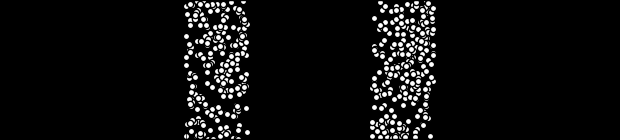
\includegraphics[width=0.6\textwidth]{particle_no_interference.png}
  \caption{Padrão observado no experimento da dupla fenda para partículas clássicas.}
  \label{fig:padrao.classico}
\end{figure}

\item Neste caso, desconsiderando o efeito da difração devido à largura das fendas, a intensidade angular após as fendas obedece, sendo $d$ a separação das fendas e $\lambda$ o comprimento de onda da onda incidente:

$$ I_{ang}(\theta) = I_{max} \cos^2\left(\pi \frac{d}{\lambda} \sin(\theta)\right). $$

Sendo $D$ a distância entre as fendas e o anteparo a intensidade na coordenada transversal do anteparo é dada por

$$ I_{lin}(z) = I\left(\arctan\left(\frac{z}{D}\right)\right). $$

A imagem observada no anteparo neste caso pode ser vista na Figura \ref{fig:padrao.ondas}.

\begin{figure}[!h]
  \centering
  
\includegraphics[width=0.6\textwidth]{wave_interference.png}
  \caption{Padrão observado no experimento da dupla fenda para ondas (clássicas).}
  \label{fig:padrao.ondas}
\end{figure}

\item Agora, sendo $\lambda$ o comprimento de onda de De Broglie dos elétrons, a densidade de probabilidade de incidência de elétrons na coordenada transversal do anteparo é proporcional à intensidade $I_{lin}$ do item anterior:

$$ p(z) \propto I_{lin}(z). $$

Plotando uma amostra de $500$ pontos cuja coordenada $x$ é amostrada da distribuição $p(z)$ e onde a coordenada $y$ segue uma distribuição uniforme obtemos a Figura \ref{fig:padrao.quantico}.

\begin{figure}[!h]
  \centering
  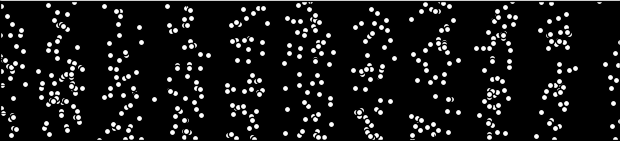
\includegraphics[width=0.6\textwidth]{particle_interference.png}
  \caption{Padrão observado no experimento da dupla fenda para partículas quânticas com comprimento de onda da ordem da separação entre as fendas.}
  \label{fig:padrao.quantico}
\end{figure}

\end{enumerate}

% Exercício 10
\addcontentsline{toc}{section}{Exercício 10}
\item (Griffiths 1.4) No tempo $t=0$ uma partícula é representada pela função de onda

\begin{equation*}
  \Psi(x, 0) = 
    \begin{cases}
    \frac{Ax}{a} &0\le x \le a\\
    \frac{A(b-x)}{(b-a)} &a \le x \le b\\
    0 &\text{qualquer outro valor}
    \end{cases}
\end{equation*}

\begin{enumerate}
  \item Normalize a função de onda $\Psi$, i.e., encontre $A$ em função de $a$ e $b$.
  \item Desenhe $\Psi(x, 0)$ como função de $x$.
  \item Qual a posição mais provável que a partícula ser encontrada em $x=0$?
  \item Qual é a probabilidade de encontrar a partícula para valores menores de $x = a$? Faça os casos limites $b=a$ e $b=2a$ e veja se o resultado tem consistência.
  \item Qual é o valor esperado de x?
\end{enumerate}

\textbf{Resolução: }\linebreak
\begin{enumerate}
  \item Impondo a normalização obtemos
  \begin{align*}
    \int_{-\infty}^{\infty} |\Psi(x,0)|^2 dx &= 1 \\
    \int_0^a A^2 \frac{x^2}{a^2} dx + \int_a^b A^2 \frac{(b-x)^2}{(b-a)^2} dx &= 1 \\
    A^2\left(\frac{1}{a^2} \frac{x^3}{3}\Big|_0^a + \frac{1}{(b-a)^2} \left(-\frac{(b-x)^3}{3}\right)\Big|_a^b\right) &= 1 \\
    A^2 \frac{\left(a + (b-a)\right)}{3} &= 1 \\
    A^2 b &= 3 \\
    A &= \sqrt{\frac{3}{b}}
  \end{align*}
  
  \item
  \hspace{0.2cm}
  \begin{figure}[!h]
    \centering
    \begin{tikzpicture}[>=latex]
		\begin{axis}[
		  samples=4000,
		  axis x line=center,
		  axis y line=center,
		  xtick={3, 7},
		  xticklabels={$a$, $b$},
		  ytick={1},
		  yticklabels={$A$},
		  xlabel={$x$},
		  ylabel={$\Psi(x)$},
		  xlabel style={below right},
		  ylabel style={above left},
		  xmin=-1,
		  xmax=8,
		  ymin=-0.5,
		  ymax=1.5]
		\addplot [mark=none,domain=-1:8] {x < 0 ? 0 : x <= 3 ? x/3 : (x <= 7 ? (7 - x)/(7 - 3) : 0)};
		\end{axis}
	\end{tikzpicture}
  \caption{Gráfico de $\Psi(x)$.}
  
  \end{figure}
  \item A posição mais provável é $x=a$, onde $|\Psi(x,0)|^2$ é máximo.
  \item A probabilidade $P(x \le a)$ corresponde à integral
  \begin{align*}
  P(x \le a) &= \int_{-\infty}^a |\Psi(x,0)|^2 dx \\
  &= \int_0^a \frac{3}{b} \frac{x^2}{a^2} dx \\
  &= \frac{3}{b}\frac{1}{a^2} \frac{a^3}{3} \\
  &= \frac{a}{b}
  \end{align*}
  Quando $b = a$ temos
  \begin{align*}
  P(x \le a) &= \frac{a}{a} \\
  &= 1
  \end{align*}
  Como esperado, já que neste caso a função de onda se anula à direita de $x=a$. Por outro lado, quando $b = 2a$ temos
  \begin{align*}
  P(x \le a) &= \frac{a}{2a} \\
  &= \frac{1}{2}
  \end{align*}
  O que também coincide com o resultado esperado (neste caso a função de onda é simétrica com relação ao eixo $x=a$).
  \item Temos
  \begin{align*}
  \left\langle x \right\rangle &= \int_{-\infty}^{\infty} x |\Psi(x, 0)|^2 dx \\
  &= \int_0^a x \left(\frac{3x^2}{a^2b}\right) dx + \int_a^b x \left(\frac{3(b-x)^2}{b(b-a)^2}\right)dx \\
  &= \frac{3}{b}\int_0^a \frac{x^3}{a^2} dx + \int_{b-a}^0 \left(b - x \right)\frac{3x^2}{b(b-a)^2}(-dx) \\
  &= \frac{3}{b}\int_0^a \frac{x^3}{a^2} dx + \int_0^{b-a} \frac{3b}{b}\frac{x^2}{(b-a)^2}dx - \int_0^{b-a} \frac{3}{b} \frac{x^3}{(b-a)^2} dx \\
  &= \frac{3}{b}\int_0^a \frac{x^3}{a^2} dx  + 3\int_0^{b-a}\frac{x^2}{(b-a)^2} dx - \frac{3}{b}\int_0^{b-a}\frac{x^3}{(b-a)^2} dx \\
  &= \frac{3}{4b} \frac{x^4}{a^2}\Big|_0^a + \frac{x^3}{(b-a)^2}\Big|_0^{b-a} - \frac{3}{4b}\frac{x^4}{(b-a)^2}\Big|_0^{b-a} \\
  &= \frac{3a^2}{4b} + (b - a) - \frac{3}{4b}\left(b^2 - 2ab + a^2\right) \\
  &= \frac{3a^2}{4b} + b - a - \frac{3b}{4} + \frac{3a}{2} -\frac{3a^2}{4b} \\
  &= \frac{2a + b}{4}
  \end{align*}
  Note que no caso em que a distribuição é simétrica, i.e., $b = 2a$, obtemos $\left\langle x \right\rangle = a$, e o valor esperado coincide com o valor mais provável da posição. Em geral, entretanto, eles diferem.
  \end{enumerate}
 
% Exercício 11
\addcontentsline{toc}{section}{Exercício 11}
\item (Griffiths 1.5) Considera a função
\begin{equation*}
\Psi(x,t) = A e^{-\lambda |x|} e^{-iw t}
\end{equation*}
\noindent onde $A$, $\lambda$ e $w$ são constantes reais e positivas.
\begin{enumerate}
  \item Normalize a função de onda $\Psi$.
  \item Determine o valor esperado de $x$ e $x^2$.
  \item Encontre o desvio padrão de $x$. Faça o gráfico de $\left|\Psi\right|^2$ como função de $x$ e indique os pontos $\left(\left\langle x \right\rangle + \sigma, \left\langle x \right\rangle - \sigma\right)$ para ilustrar o sentido que $\sigma$ representa a incerteza de $x$. Qual a probabilidade de a partícula ser encontrada fora deste intervalo?
\end{enumerate}

\textbf{Resolução: }\linebreak
\begin{enumerate}
  \item 
  \begin{align*}
  \int_{-\infty}^{\infty} |\Psi(x,t)|^2 dx &= 1\\
  \int_{-\infty}^{\infty} A^2 e^{-2\lambda |x|} dx &= 1 \\
  2A^2\int_0^\infty e^{-2\lambda x} dx &= 1 \\
  2A^2\frac{-1}{2\lambda}\left(e^{-2\lambda x}\right) \Bigg|_0^{\infty} &= 1 \\
  \frac{2A^2}{2\lambda} &= 1 \\
  A &= \sqrt{\lambda}
  \end{align*}
  
  \item Para o valor esperado de $x$ temos
  \begin{align*}
  \left\langle x \right\rangle &= \int_{-\infty}^{\infty}x \lambda e^{-2\lambda |x|} dx \\
  &= 0
  \end{align*}
  Já para o valor esperado de $x^2$
  \begin{align*}
  \left\langle x^2 \right\rangle &= \int_{-\infty}^{\infty}x^2 \lambda e^{-2\lambda |x|} dx \\
  &= 2\lambda\int_{0}^{\infty}x^2 \lambda e^{-2\lambda x} dx \\
  &= \frac{\lambda}{2} \int_0^{\infty} \frac{\partial^2}{\partial \lambda^2} e^{-2\lambda x} dx \\
  &= \frac{\lambda}{2} \frac{d^2}{d\lambda^2} \int_0^{\infty} e^{-2\lambda x} dx \\
  &= \frac{\lambda}{2} \frac{d^2}{d\lambda^2} \left(\frac{1}{2\lambda}\right) \\
  &= \frac{\lambda}{2} \left(\frac{1}{\lambda^3}\right) \\
  &= \frac{1}{2\lambda^2}
  \end{align*}
  \item Como $\sigma^2 = \left\langle x^2 \right\rangle - \left\langle x \right\rangle ^2$ temos
  \begin{equation*}
  \sigma = \frac{1}{\sqrt{2}\lambda}
  \end{equation*}
  
  A densidade de probabilidade é então dada por
  
  \begin{equation*}
  |\Psi(x,t)|^2 = \lambda e^{-2\lambda |x|}.
  \end{equation*}
  
  O gráfico desta função (para $t$ constante) pode ser visto na Figura \ref{fig:psi2}.
  
  \begin{figure}[!h]
    \centering
    % Densidade de probabilidade para desvio padrão unitário
    \def\FunctionPsi(#1){1/sqrt(2) * exp(-sqrt(2)*abs(#1))}
    \begin{tikzpicture}[>=latex]
		\begin{axis}[
		  samples=400,
		  axis x line=center,
		  axis y line=center,
		  xtick={-1, 1},
		  xticklabels={$-\sigma$, $+\sigma$},
		  ytick={0.707},
		  yticklabels={$\lambda$},
		  xlabel={$x$},
		  ylabel={$\left|\Psi(x)\right|^2$},
		  xlabel style={below right},
		  ylabel style={above left},
		  xmin=-2.5,
		  xmax=2.5,
		  ymin=-0.5,
		  ymax=1]
		\addplot [smooth, name path=A] {\FunctionPsi(x)};
		\addplot [draw=none, name path=B] {0};
		\addplot [gray!30] fill between[of=A and B, soft clip={domain=-1:1}];
		\end{axis}
	\end{tikzpicture}
  \caption{Gráfico de $|\Psi(x)|^2$.}
  \label{fig:psi2}
  \end{figure}
  
  A probabilidade de a partícula ser encontrada fora do intervalo $\left(\left\langle x \right\rangle - \sigma, \left\langle x \right\rangle + sigma\right)$ é dada por
  
  \begin{align*}
  \int_{-\infty}^{-\sigma} |\Psi(x)|^2dx + \int^{\infty}_{\sigma} |\Psi(x)|^2dx &= 1 - \int_{-\sigma}^{\sigma} |\Psi(x)|^2 dx \\
  &= 1 - \int_{-\sigma}^{\sigma} \lambda e^{-2\lambda |x|} dx \\
  &= 1 - 2\lambda\int_0^{\sigma} e^{-2\lambda x} dx \\
  &= 1 - 2\lambda \frac{e^{-2\lambda x}}{-2\lambda} \Big|_0^{\sigma} \\
  &= 1 + e^{-2\lambda \sigma} - 1 \\
  &= e^{-2\lambda \frac{1}{\sqrt{2}\lambda}} \\
  &= e^{-\sqrt{2}} \\
  &= 0.243.
  \end{align*}
  
\end{enumerate}

% Exercício 12
\addcontentsline{toc}{section}{Exercício 12}
\item Seja o poço infinito. Em vez da solução dada na Equação 2.28 do Griffiths, página 32, assuma que a solução é
\begin{equation*}
\psi(x, t) = C e^{ikx} + D e^{-ikx}
\end{equation*}

\begin{enumerate}
  \item Refaça o problema assumindo esta solução. Ache as energias e as funções de onda deste problema.
\end{enumerate}

\textbf{Resolução: }\linebreak
\begin{enumerate}
  \item Considerando o potencial
  \begin{equation*}
  V(x) = \begin{cases} 0 &0 < x < a \\ 
  \infty &\text{caso contrário.}
  \end{cases}
  \end{equation*}
  \noindent temos para $\psi(x, t)$ as condições de contorno $\psi(0, t) = \psi(a, t) = 0$ que fornecem
  \begin{align*}
  \psi(0, t) &= 0 \\
  C + D &= 0\\
  C &= -D
  \end{align*}
  \noindent e, já substituindo a condição anterior na definição de $\psi(x,t)$,
  \begin{align*}
  \psi(a, t) &= 0\\
  C\left(e^{ika} - e^{-ika}\right) &= 0 \\
  \sin(ka) &= 0.
  \end{align*}
  Concluímos então que os valores permitidos de $k$ são
  \begin{equation*}
  k_n = \frac{n\pi}{a}\qquad\text{para }n \in \{1, 2, 3,\ldots\}.
  \end{equation*}
  Para encontrar as funções de onda $\Psi_n(x, t) = C\left(e^{ik_nx} - e^{-ik_n x}\right)$ (para $x \in [0, a]$) resta-nos apenas encontrar a constante de normalização $C$.
  \begin{align*}
  1 &= \int_{-\infty}^{\infty} \left| \Psi(x,t)\right|^2 dx \\
  1 &= \left| C\right|^2 \int_0^a \left(e^{ik_nx} - e^{-ik_nx}\right)\left(e^{-ik_nx} - e^{ik_nx}\right) dx \\
  1 &= \left| C\right|^2 \int_0^a \left(2 - \left(e^{2ik_nx} + e^{-2ik_nx}\right)\right) dx \\
  1 &= 2\left| C\right|^2 \int_0^a \left(1 - \cos(2k_n x)\right) dx \\
  1 &= 2\left| C\right|^2 \left(a - \frac{\sin(2k_nx)}{2k_n}\Big|_0^a\right) \\
  1 &= 2\left| C\right|^2 a \\
  \left| C \right| &= \sqrt{\frac{1}{2a}}.
  \end{align*}
  A menos de fases imaginárias, irrelevantes para medidas físicas, as funções de onda do problema são
  \begin{equation*}
  \Psi_n(x, t) = \sqrt{\frac{1}{2a}} \left( e^{i\frac{n\pi}{a}} - e^{-i\frac{n\pi}{a}}\right)\qquad\text{para }n \in \{1, 2, 3, \ldots\}.
  \end{equation*}
  Para encontrar as energias basta substituir as funções encontradas na equação de Schrödinger independente do tempo:
  \begin{align*}
  E_n \Psi_n &= -\frac{\hbar^2}{2m}\frac{d^2 \Psi_n}{dx^2} \\
  &= \frac{\hbar^2}{2m}\left(\frac{n\pi}{a}\right)^2\sqrt{\frac{1}{2a}}\left(e^{i\frac{n\pi}{a}} - e^{-i\frac{n\pi}{a}}\right) \\
  &= \frac{h^2}{8m\pi^2}\left(\frac{n\pi}{a}\right)^2 \Psi_n \\
  &= \left(\frac{(nh)^2}{8ma^2}\right) \Psi_n \\
  \end{align*}
  As energias permitidas são portanto dadas por
  \begin{equation*}
  E_n = \frac{(nh)^2}{8ma^2}.
  \end{equation*}
  Alternativamente, sendo $k_n$ os números de onda permitidos dentro do poço, os momentos associados, dados pelas relações de De Broglie, são $p_n = \hbar k_n$, logo as energias associadas são $E_n = 1/2m \left(\hbar k_n\right)^2$. Substituindo $k_n = n\pi/a$ obtemos $E_n = n^2 h^2/(8ma^2)$.
\end{enumerate}

% Exercício 13
\addcontentsline{toc}{section}{Exercício 13}
\item (Griffiths 2.2) Mostre que $E$ precisa ser maior do que o valor mínimo de $V(x)$ para cada solução normalizável da equação de Schrodinger independente do tempo.
\begin{enumerate}
  \item Qual é o análogo clássico deste teorema?
  \item Reescreva a Equação 2.5 do Griffiths na forma,
  \begin{equation*}
  \frac{d^2 \Psi}{dx^2} = \frac{2m}{\hbar^2}\left(V(x) - E\right)\Psi
  \end{equation*}
  Se $E < V_{min}$ então $\Psi$ e a segunda derivada precisam ter sempre o mesmo sinal, e argumente que tal função não pode ser normalizada.
\end{enumerate}
\textbf{Resolução: }\linebreak
\begin{enumerate}
  \item É a constatação de que a energia mecânica de uma partícula é sempre maior que o potencial onde a partícula está, e que portanto as únicas regiões acessíveis a uma partícula são aquelas onde a energia da partícula é maior que o potencial.

  \item A equação de Schrödinger independente do tempo em uma dimensão é

$$ -\frac{\hbar^2}{2m} \frac{d^2 \Psi}{dx^2} + V \Psi = E\Psi(x). $$

  Isolando a derivada segunda de $\Psi(x)$ temos

$$ \frac{d^2\Psi}{dx^2} = \frac{2m}{\hbar^2}\left(V - E\right)\Psi. $$

  Sendo $V_{min}$ o valor mínimo de $V(x)$, se $E < V_{min}$ é claro que $V(x) - E \ge V_{min} - E > 0$, logo na equação acima notamos que tanto as partes imaginárias quanto as reais de $d^2\Psi/dx^2$ e $\Psi$ sempre possuem o mesmo sinal. Como a derivada segunda mede a concavidade/convexidade de uma função, isto significa que se os gráficos de $\text{Re}(\Psi)$ e $\text{Im}(\Psi)$ em algum momento se afastarem do eixo $x$ (o que necessariamente deve ocorrer para que as integrais $\left(\text{Re}(\Psi)\right)^2$ e $\left(\text{Im}(\Psi)\right)^2$ não se anulem), eles se curvariam para fora do eixo $x$, e portanto se afastariam deste eixo nos limites $x \rightarrow \pm \infty$ (cf. Figura \ref{fig:ilustracao.concavidade}), fazendo com que as integrais citadas não sejam convergentes. Isto implica que a integral  $\int_{-\infty}^{\infty}|\Psi(x)|^2dx = \int_{-\infty}^{\infty}\left(\text{Re}\left(\Psi(x)\right)\right)^2 + \left(\text{Im}\left(\Psi(x)\right)\right)^2 dx$ é nula ou não converge, logo a função de onda não pode ser normalizável.


  \begin{figure}[!h]
    \centering
    \begin{tikzpicture}[>=latex]
	    \begin{axis}[
	       samples=500,
	       axis x line=center,
	       axis y line=center,
	       xlabel={$x$},
	       ylabel={$f(x)$},
	       xlabel style={below right},
	       ylabel style={above left},
         ticks=none,
		     xmin=-10,
		     xmax=10,
		     ymin=-10,
		     ymax=10]
		     \addplot [mark=none,domain=-10:10] {0.05*(x^2 + 20)} node [above left] {$f(x) > 0$};
		     \addplot [mark=none,domain=-10:10] {-0.1*((x-4)^2 + 20)} node [below left] {$f(x) < 0$};
		   \end{axis}
    \end{tikzpicture}
	  \caption{Ilustração de como a concavidade/convexidade de uma função $f$ impede que $\lim_{x \to \pm \infty} f(x) = 0$.}
	  \label{fig:ilustracao.concavidade}
  \end{figure}
\end{enumerate}

  \textbf{Bônus:} Abaixo segue uma demonstração mais formal de que as partes reais e imaginárias de $\Psi$ não podem ser normalizáveis. Não é necessário argumentar neste nível de rigor neste problema, mas o argumento pode ser interessante aos mais céticos.

  \begin{lema}\label{lema:lema1}
    Seja $f: \R \rightarrow \R$ função duas vezes derivável tal que existe $g: \R \rightarrow \R_+$ com $f'' = g\cdot f$. Se $a_1 < a_2$ são duas raízes de $f$, $f(x) = 0$ para todo $x \in [a_1, a_2]$.
  \end{lema}
  \begin{proof}
    O teorema do valor extremo garante que existem $b_+$ e $b_-$ em $[a_1, a_2]$ tais que $f(b_+)$ é o máximo e $f(b_-)$ o mínimo de $f$ neste intervalo. Se $f(b_+) > 0$ então $b_+ \in (a_1, a_2)$ e $f'(b_+) = 0$. Mas $f''(b_+)$ tem o mesmo sinal de $f(b_+)$, logo $f''(b_+) > 0$ e $b_+$ é mínimo local de $f$. Conclui-se então que $f$ é localmente constante em $b_+$, mas isto implica $f''(b_+) = 0$, e desta contradição concluímos que o valor máximo de $f$ em $[a_1, a_2]$ é $0$. Argumento análogo mostra que o valor mínimo de $f$ no mesmo intervalo é $0$, logo $f(x) = 0$ para todo $x$ em $[a_1, a_2]$.
  \end{proof}
  \begin{teorema}
    Seja $f: \R \rightarrow \R$ função duas vezes derivável tal que existe $g: \R \rightarrow \R_+$ com $f'' = g\cdot f$. $f^2$ não é normalizável (i.e., a integral $\int_{-\infty}^{\infty} f^2(x)dx$ não converge para um valor não nulo).
  \end{teorema}
  \begin{proof}
    Separamos a demonstração em dois casos:
    \begin{itemize}
      \item $f(x) \neq 0$ para todo $x \in \R$.
    
      Neste caso o sinal de $f$ é constante, suponha sem perda de generalidade positivo. Então $f$ é convexa. Seja $a \in \R$ qualquer. Se $f'(a) \ge 0$ é impossível que $\lim_{x \to \infty} f(x) = 0$, pois, por convexidade, o gráfico de $f$ deve ficar acima da reta tangente a $f$ por $(a, f(a))$. Se $f'(a) < 0$ então é impossível que $\lim_{x \to -\infty} f(x) = 0$ por argumento análogo. É claro portanto que a integral de $f^2$ em $\R$ não converge.
    
      \item Existe $b \in \R$ tal que $f(b) = 0$.
    
      Assumindo que $f$ não é identicamente nula em toda a reta (caso na qual $f^2$ trivialmente é não normalizável), como pelo Lema \ref{lema:lema1} $f$ é identicamente nula entre duas raízes, neste caso existe $c$ suficientemente grande tal que $f(c) = 0$ e $f(x) \neq 0$ para $x \in (c, \infty)$ ou $f(-c) = 0$ e $f(x) \neq 0$ para $x \in (-\infty, -c)$. Sem perda de generalidade nos restringiremos ao primeiro caso, e suporemos $f(x) > 0$ para $x \in (c, \infty)$. Neste caso $f$ restrita a este intervalo é convexa. Supondo por absurdo que $\lim_{x \to \infty} f(x) = 0$ existem secantes ao gráfico de $f$ restrita ao intervalo $(c, \infty)$ arbitrariamente próximas do eixo $x$. Por convexidade portanto o gráfico de $f$ deve estar abaixo do eixo $x$, o que é absurdo. Como a hipótese que $\lim_{x \to \infty} f(x) = 0$ é falsa concluímos que a integral de $f^2$ na reta não pode convergir, logo $f^2$ não é normalizável.
    \end{itemize}
  \end{proof}

%FIM DOS EXERCÍCIOS
\end{enumerate}
\end{document}
